\documentclass[12pt,a4paper,notitlepage]{article}
% \documentclass[conf]{new-aiaa}
\usepackage[framed,numbered,autolinebreaks]{mcode}
\usepackage[margin=1in]{geometry}
\usepackage{amsmath}
\usepackage{amsfonts}
\usepackage{amssymb}
\usepackage{graphicx}
\usepackage{color}
\usepackage{float}
\usepackage[toc,page]{appendix}
\usepackage{parskip}
\usepackage{sectsty}
\usepackage{gensymb}
\usepackage{titlesec}
\usepackage{listings}
% \lstset{language=Matlab,%
%     %basicstyle=\color{red},
%     breaklines=true,%
%     morekeywords={matlab2tikz},
%     keywordstyle=\color{blue},%
%     morekeywords=[2]{1}, keywordstyle=[2]{\color{black}},
%     identifierstyle=\color{black},%
%     stringstyle=\color{mylilas},
%     commentstyle=\color{mygreen},%
%     showstringspaces=false,%without this there will be a symbol in the places where there is a space
%     numbers=left,%
%     numberstyle={\tiny \color{black}},% size of the numbers
%     numbersep=9pt, % this defines how far the numbers are from the text
%     emph=[1]{for,end,break},emphstyle=[1]\color{red}, %some words to emphasise
%     %emph=[2]{word1,word2}, emphstyle=[2]{style},    
% }
\usepackage{titling}
\setlength{\droptitle}{-1cm}
\usepackage{enumitem}
\usepackage{multirow}
\usepackage{longtable}

\usepackage[
backend=biber,
style=numeric,
sorting=none
]{biblatex}
 
\addbibresource{draft.bib}


\setlist[enumerate]{topsep=0pt,itemsep=-3.5ex,partopsep=1ex,parsep=1ex}
\renewcommand{\rmdefault}{ptm}
\sectionfont{\fontsize{12}{0}\selectfont}
\subsectionfont{\fontsize{12}{0}\selectfont}
\usepackage[font={normal,bf}]{caption}

% Header and Footer
\setlength{\headheight}{15pt} 
\usepackage{fancyhdr}
\fancypagestyle{plain}{
 \fancyhf{}
 \fancyhead[L]{AA 290: AA 279D Project}
 \fancyhead[R]{Stanford University}
 \fancyfoot[C]{\thepage}
}

% Table of contents
\setcounter{tocdepth}{5}

\begin{document}
\title{\Huge \textbf{Project Title}}
\author{\Large Ethan LeBoeuf}
\date{\Large 23 September 2019}

\begin{minipage}[h]{\textwidth}
	\vspace{4 cm}
	\advance\leftskip-1in
    \maketitle
\end{minipage}

\begin{figure}[H]
\centering
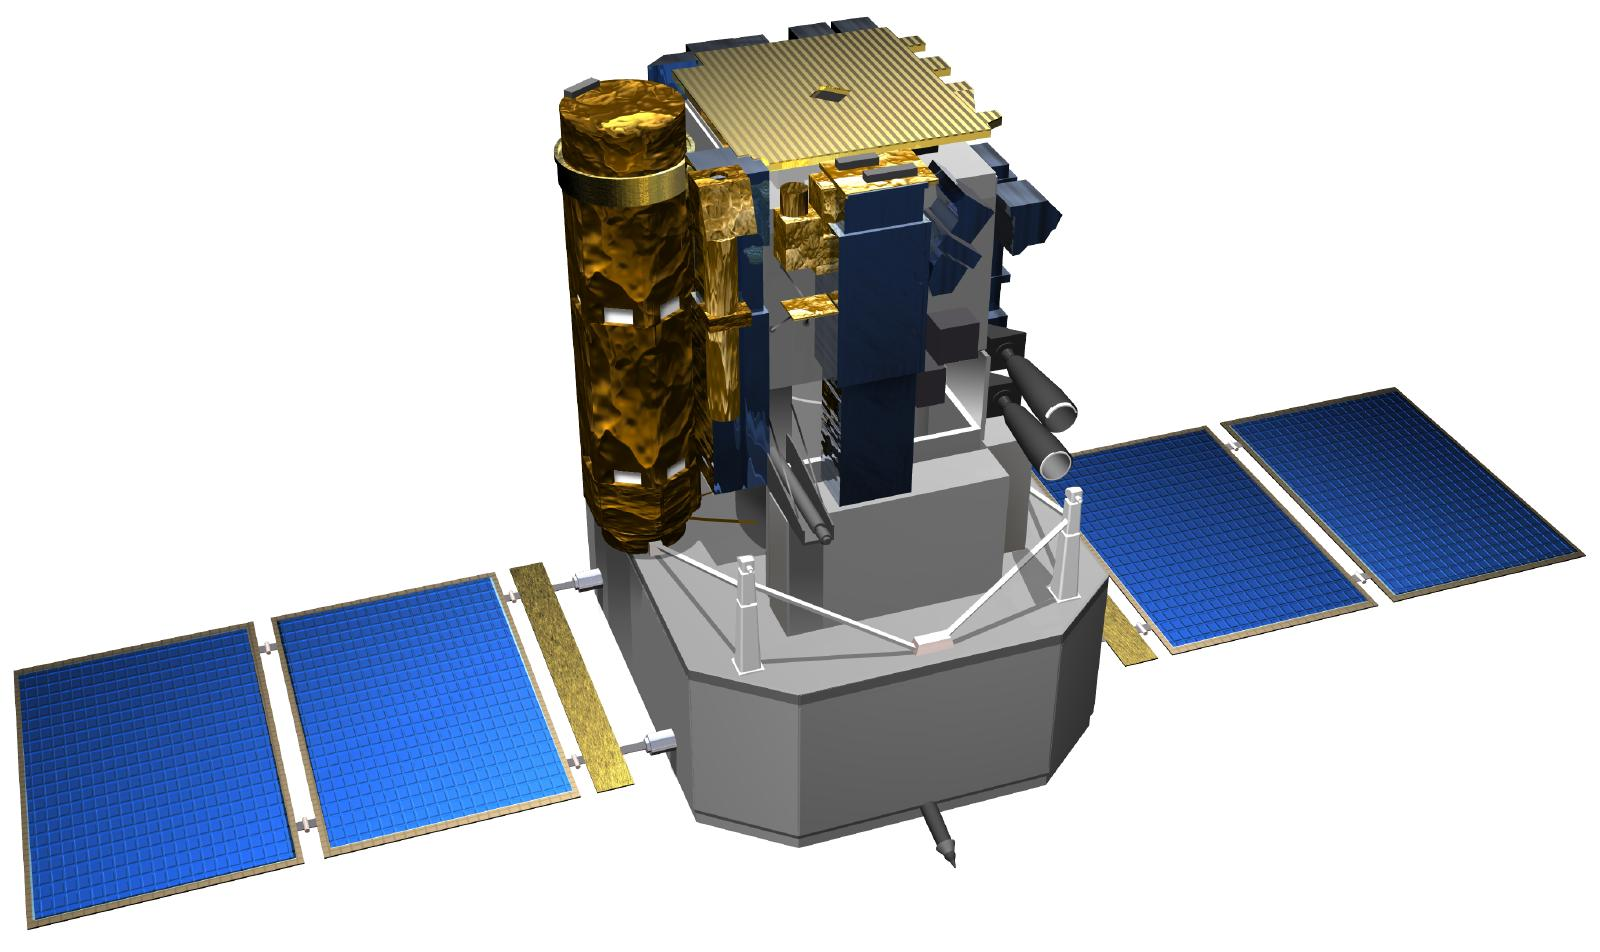
\includegraphics[scale=0.28]{Images/SOHO.jpg}
\end{figure}

\pagebreak

\section*{\Large REVISION HISTORY}

\begin{table}[h!]
\begin{center}
\begin{tabular} [0.9 \textwidth]{cl}
\hline \hline
\multicolumn{1}{c}{VERSION} & \multicolumn{1}{l}{REVISION NOTES} \\
\hline
PS1 & - Created document \\
    & - Added PS1 material \\
%  \hline
%  PS2 & - Added PS2 material \\
%  & - Updated title page \\
%  & - Added table of contents \\
%  & - Updated orbit around L2 point \\
%  & - Discretized cylindrical parts of geometry \\
\hline \hline
\end{tabular}
	\caption{Summary of project revisions.}
\end{center}
\end{table}
 
\newpage
\section*{\Large TABLE OF CONTENTS}
\makeatletter
\@starttoc{toc}
\makeatother
\newpage
%%%%%%%%%%%%%%%%%%%%%%%%%%%%%%%%%%%%%%%%%%%%%%%%%%%%%%%%%%%%%%%%%%%%%%%%%%%%%%%%%%%%%%%%%%%%%%%%%%%%%%%%%%%%%%%%%%%%%%%%%%%%%%%%%%%%%%%%%%%%%%%%%%%%%%%%%%%%%%%%%%%%%%%%%%%%%%%%%%%%%%%%%%%%%%%%%%%%%%%%%%%%%%%%%%%%%%%%%%%

% \section{\Large INTRODUCTION}

\section{\Large PROBLEM SET 1}
\subsection{PROBLEM 1}
Current Ideas:
RSGS, Restore-L, Orbital Re-supply, Orbital Express
Look into telescopes/aperatures

\newpage
\printbibliography

\newpage
\appendix
\addappheadtotoc
\Large{\bf{\appendixname}}
\section{Matlab Code}
\subsection{PSet1 Problem 5}\label{A:P1p5}

\lstinputlisting{test.m}



\end{document}